\chapter{绪论}
\section{引言}
文字和语音一直都是自然语言处理领域的研究对象。无论是比较早期的句法、词法分析,音素和发声研究,还是诞生稍晚的针对语音内容的识别、拼接合成等,对于文字和语音内容的研究可称得上互为表里。语音是文字可感知的信号载体、是人类使用最频繁、最自然的``通信接口''之一,文字则是语音内容的本质表示。

机器翻译一直以来都是自然语言处理领域针对不同语言文字的一项重要技术。对于机器翻译的研究最早始于20世纪30年代,它的发展一直与计算机技术、语言学和信息论等学科密切相关。从早期的字典匹配、结合专家知识的规则翻译等朴素方法,到结合概率统计学和语言学的统计机器翻译,再到近年来随着运算硬件性能提高和深度神经网络发展而兴起的神经机器翻译,机器翻译技术取得了世人瞩目的成功,这项技术本身也逐渐从学界中的理论发展走向工业界的落地实践。
自动歌曲翻译是神经机器翻译在这一基础上针对非常规语体的拓展性研究,这一任务旨在快速地、自动地、高质量地将歌曲的歌词文本翻译到另外一种语言中,同时要求翻译后歌词文本搭配相应旋律依然能以歌曲的形式呈现出来,即翻译后歌词仍能以某种方式来进行艺术性的演唱并传达原意。除了歌词近似诗词的语体问题以外,这样的翻译也相比于一般的机器翻译任务增加了一项需要考虑的旋律乐谱信息。

语音合成任务旨在将文字合成为可理解的自然语音,是一个比翻译更加多元的任务。
语音合成研究需要自然语言处理和人类发声的知识,涉及多个学科,包括语言学、声学、数字信号处理等。
歌声合成(Singing Voice Sythesis,SVS)任务则是由语音合成任务衍生而来。语音合成是仅以文本为输入、以梅尔频率特征图谱或直接以声波波形为输出的生成任务,歌声合成和语音合成任务不同的是,其文本发声时所对应的音高和时长都为设定好的乐谱所限制。
歌声合成使得直观地呈现歌曲翻译结果成为可能。同时,由于歌声合成可以承接歌曲翻译的输出而连接成为完整的级联式歌曲到歌声的翻译系统,这为歌曲翻译的实际应用打下了坚实的基础。自动歌曲翻译搭配良好的歌声合成效果进行翻唱自动合成,那么听众无需学习多国语言、乐理知识或具备演唱能力就能欣赏来自不同语言不同文化的经典歌曲的母语翻唱版本。
\section{国内外研究现状}
\subsection{自动歌曲翻译国内外研究现状}
歌曲翻译作为人工翻译子任务的研究历史很长,语言学领域对此任务也有体系化的研究。但当自然语言和翻译研究进入深度学习时代时,自动化歌曲翻译研究却相对发展缓慢,目前仅有极少量工作\citep{gagast}对这一方向进行过探讨。此外,翻译领域如WMT14、WMT16等多语言翻译公开数据集层出不穷,但涉及词曲类的公开翻译语料则非常寥寥。歌曲本身的电子化需要有一定专业知识的人员完成,即使借助于神经网络模型,在实际错误率较高的情况下也需要人员校对,因此研究本身就具有一定的门槛。在充分感受、理解歌曲的基础上进行的翻译则更有难度。
\subsection{歌声合成国内外研究现状}
近年来,随着深度学习研究和硬件发展,歌声合成技术因其产生自然而富有表现力的歌声的潜力而越来越受到研究界和娱乐行业的关注。歌声合成技术使用的模型的一种基本框架是一种由两种模型构成的两阶段方法~\citep{nakamura2019singing,lee2019adversarially,blaauw2020sequence,ren2020deepsinger,chen2020hifisinger}。两个模型通常由一个声学模型和一个声码器组成,这个声学模型用于根据歌谱包含的歌词、音符音调和音符时值信息生成声学特征(例如梅尔频谱)供声码器使用,该声码器用于将声学模型产生的声学特征转换为波形。

在以往研究中,声学模型这一部分主要利用一些简单的损失函数(例如L1,即一范数;或L2,即二范数)来重构声学特征。然而,基于简单损失函数的优化基于不正确的单峰分布假设,所以会导致输出的频谱有模糊和过度平滑的问题。尽管现有方法试图通过生成对抗训练(GAN)~\citep{lee2019adversarially,chen2020hifisinger}来解决此问题,但由于对抗训练的交替更新和鉴别器训练稳定性问题,这样的对抗训练经常失败,很不稳定,需要较多人力参与调整。这些问题阻碍了歌声合成的发展。

最近,有一类高度灵活且易于处理的生成模型研究崭露头角,即扩散概率模型(也称扩散模型)~\citep{sohl2015deep,Ho2020ddpm,song2021denoising}。扩散模型由两个过程组成:扩散过程和反向过程(也称为去噪过程),扩散过程是一个具有固定参数的马尔可夫链,它通过逐渐添加高斯噪声将复杂数据转换为高斯分布;而反向过程是由神经网络实现的马尔可夫链,用于学习从高斯白噪声中迭代地恢复为原始数据的去噪过程。通过隐式地优化数据似然的变分下界(Evidence Lower Bound,ELBO),扩散模型可以稳定地进行训练。现有最新工作证明,扩散模型可以在图像生成~\citep{Ho2020ddpm,song2021denoising}和神经声码器~
\citep{chen2021wavegrad,kong2021diffwave}这样的生成任务中取得很有潜力的实验结果。

基于以上考虑,本文以歌声合成音频质量提升和实际应用为目标,研究基于扩散模型构建声学模型的技术方案,以克服之前工作提出的做法的局限和问题。
\section{本文工作的研究内容及意义}
歌曲翻译技术是人类为了攀登更高层次的跨文化交流之巴别塔而做出的很有意义的技术努力。
\begin{figure}[htbp]
  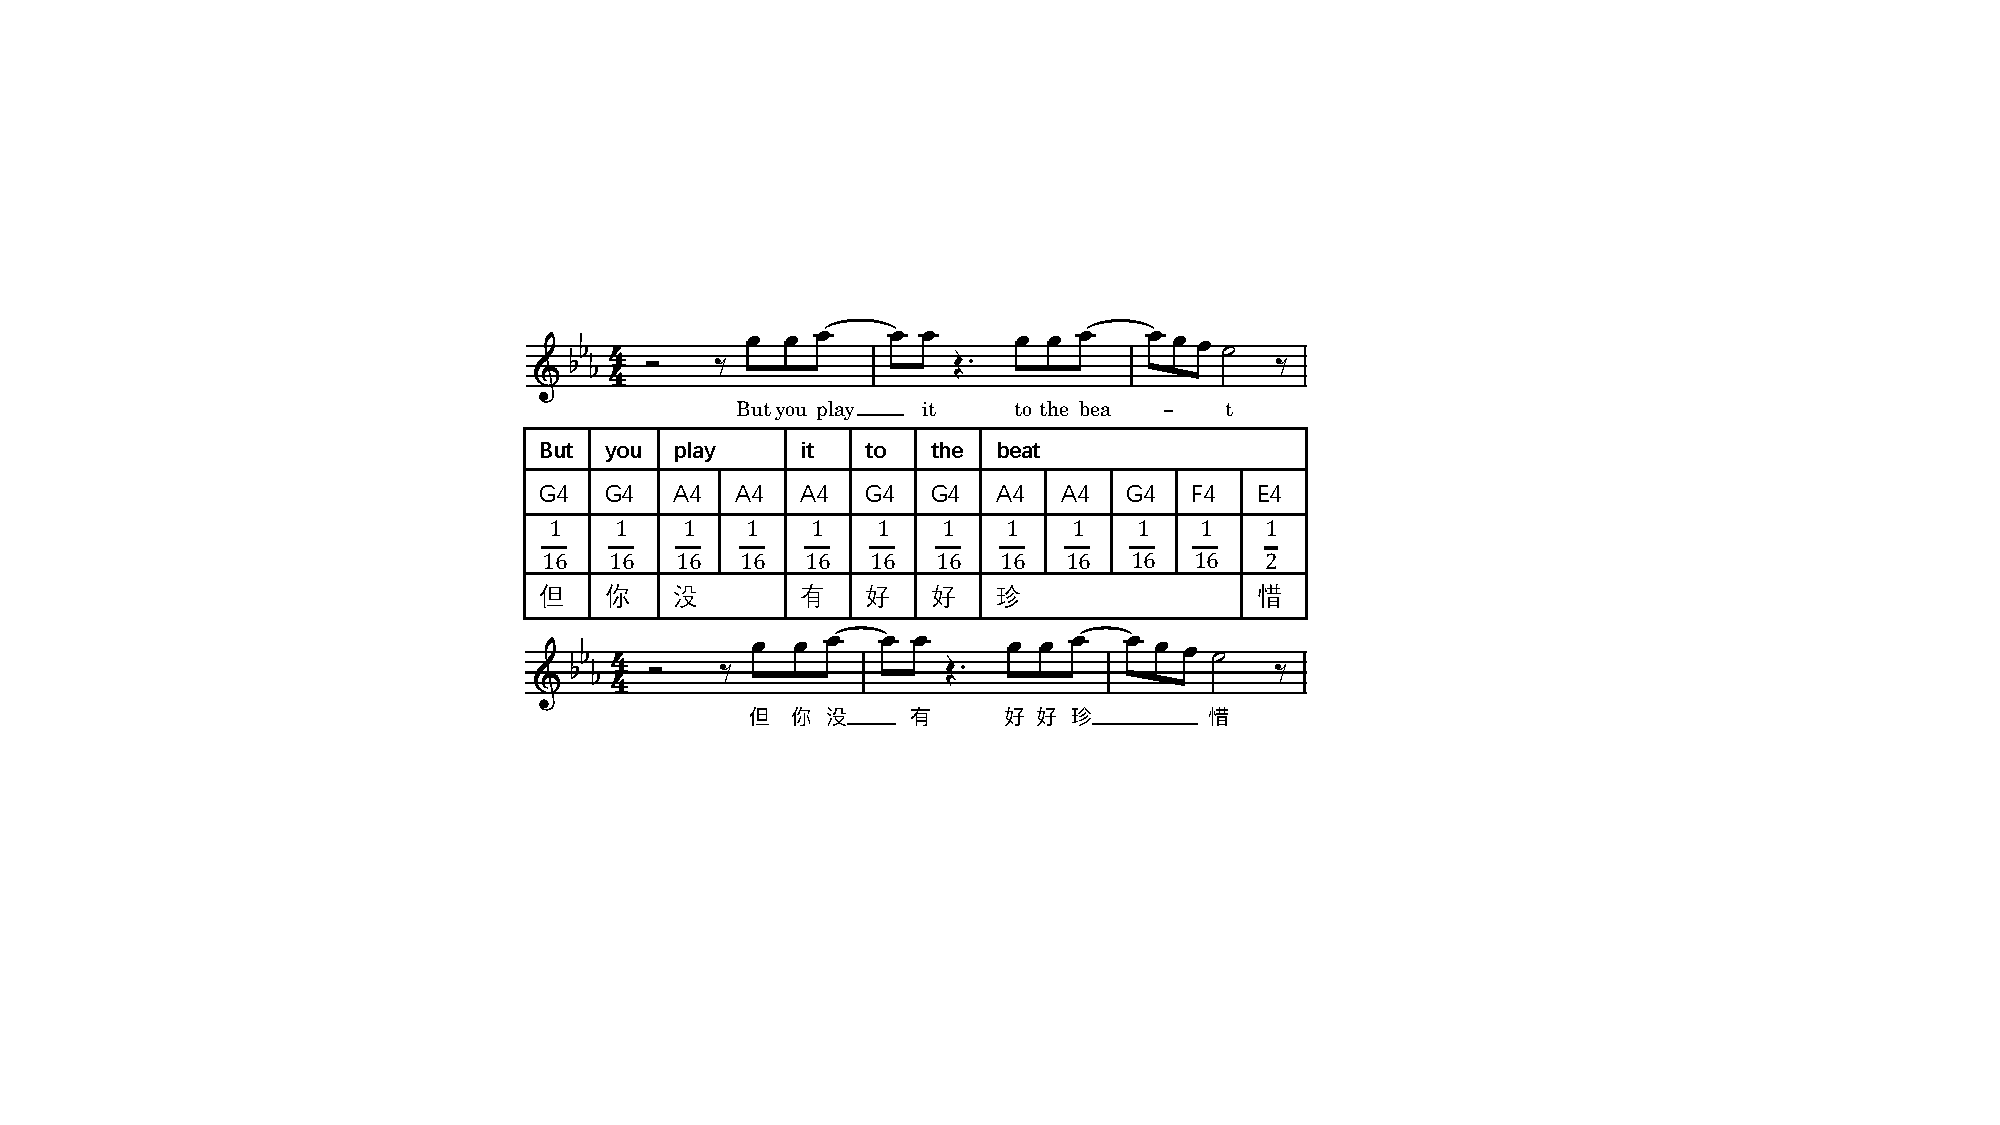
\includegraphics[width=0.99\textwidth]{figure/ast/exp.pdf}
  \caption{以\textit{Rolling In the Deep}一曲中``But you play it to the beat''一句的完整歌曲翻译为例。}
  \label{fig:task_exp}
\end{figure}
然而,尽管机器翻译(Machine Translation,MT)技术,尤其是神经机器翻译~\citep{nmt,vaswani2017attention,hassan2018achieving}(Neural Machine Translation,NMT)自诞生以来已经取得了长足进步,也吸引了许多领域研究者投身其中,自动歌曲翻译在自然语言处理学界中却并未得到充分的研究探索。这其中客观存在的一些挑战包括缺乏收集平行歌词和对齐数据的高效方式、难以对文本和旋律之间的复杂交互进行建模以及没有对乐谱规定的演唱方式进行直观评估的方式。歌曲翻译虽然与文本翻译密切相关,但本质上是一项更复杂的任务。除了在翻译中如用词和词序这样的语体问题带来的额外翻译考虑之外,歌曲的人工翻译者还需要具有目标语言的背景,能理解源语言并作出目标语言中诗意化的表达。此外,如图\ref{fig:task_exp}所示,翻译的歌词需要与旋律合理地对齐来保持歌曲的美感,这是歌曲翻译中不可缺少的要素~\citep{three_d_of_singability}。高质量的歌声合成效果应能细致地预测出谐波间的细节、准确地建模人声的高频部分以达到体现人声特点、突出高音和共鸣等艺术感的歌声效果。

此前,如前节所述,学界也探索过歌声合成这一技术来自动化地合成歌曲的人声演唱,并提出了一些在给定歌词和歌谱的情况下产生具有真实人声音色的、自然的、准确的歌声的方法。这样的方法不但使得对歌曲翻译结果方便而直观的评估成为可能,而且也为自动写歌谱曲、自动歌曲翻译这样的研究任务的实际落地奠定了基础。然而,自动歌曲翻译方向上的研究和歌声合成相比很少,也未有工作探索过为歌曲翻译结果进行的翻唱歌声合成。作为目前为数不多的工作之一,\citet{gagast}专注于通过在神经机器翻译的推理过程中施加特定约束来匹配有声调语言的翻译目标词语和旋律的音调、节奏等来得到更加合适、不易造成误解的翻译歌词。然而,这篇工作直接使用文本翻译模型并对音符和字符之间对齐的严格规定一对一的匹配,无法捕捉到歌曲翻译更复杂的本质——即歌词和歌词-旋律对齐之间的关系。虽然音符的数量可以当作是翻译长度的一个简单上限,但正如\citet{interplay_lyrics_melody}一文中所观察到的现象,歌词和旋律之间的微妙对齐不应仅为简单而严格的规则所决定。针对翻唱的歌声合成也需兼容翻译结果,并提升合成质量以求达到与原端相匹配的翻唱合成效果。

为了解决上述技术挑战,本文提出了带有自适应分组的歌词-旋律共同翻译模型,这是自动歌词翻译问题的第一个完整的技术解决方案,通过在基于Transformer的编码器-解码器框架内对歌词翻译和歌词-旋律对齐进行联合建模,本文提出的模型翻译出的歌曲既忠实于原歌词,又符合旋律,无论是客观指标还是主观评测都显示出模型翻译表现的优越性。为了承接共同翻译模型的翻唱结果输出,自动地、快速地合成良好的翻唱歌声,本文提出了基于扩散模型和对抗训练的歌声合成声学模型以求高质量地自动合成歌曲翻译的翻唱结果。
\section{章节安排}
本文分为5个章节展开,各章节组织如下:

第1章:绪论。第一章节介绍了本文主要研究内容,即自动歌曲翻译技术和歌声合成技术的定义、应用和发展情况、自动歌曲翻译和歌声合成的国内外研究现状、以及自动歌曲翻译和歌声合成的研究背景及意义。另外,第一章节还阐述了本文将基于Transformer的编码器-解码器模型和歌词和歌词-旋律对齐的关系来研究自动歌曲翻译任务、基于扩散模型来研究歌声合成任务,并探究本章提出的音乐、轻量级对齐模块对于自动歌曲翻译和扩散模型、浅扩散机制对于歌声合成效果的影响。

第2章:相关研究介绍。第二章节分两部分分别介绍了本文所研究内容的相关技术综述,包括自动歌曲翻译技术所涉及的歌词生成、限制性翻译、歌词对齐预测和歌声合成技术涉及的声学模型以及扩散模型。

第3章:自动歌曲翻译研究。第三章节主要介绍本文提出的一种能很好适配基于Transformer的编码器-解码器的自回归神经机器翻译框架的歌词和歌词-旋律对齐共同翻译模型,介绍本文提出的针对歌词翻译任务的音符嵌入表示模块和对齐解码器,以及详细叙述模型结构和设计,最后介绍本文的数据来源和数据集构建方式、数据预处理方法、实验中的超参数,并展示本文提出的翻译模型其它类似模型的对比实验结果和模块消融实验结果。

第4章:翻唱歌声自动合成研究。第四章节主要介绍本文提出的基于扩散模型和对抗训练构建的声学模型,以及详细叙述模型结构和设计,最后介绍本文的数据来源和数据集构建方式、数据预处理方法、实验中的超参数,并展示本文提出的声学模型和其它声学模型的对比实验结果和模块消融实验结果。

% 第五章:歌曲到歌声翻译系统实践。
第5章:总结和展望。第五章总结了本文的主要研究内容,指出本文进行的研究的不足之处,讨论在本文探讨的自动歌曲翻译技术和翻唱自动合成技术工作基础上可进一步研究的方向。
\section{章节小结}
本章主要介绍了自动歌曲翻译技术和歌声合成技术的定义、意义和重要性,并简要地阐述了国内外现有方法的不足之处和本文工作的内容和意义。
